\chapter{Convolutional Neural Networks}
\label{chap-cnn}

So far, we have studied what are called {\em fully connected} neural
networks, in which all of the units at one layer are connected to all
of the units in the next layer. This is a good arrangement when we
don't know anything about what kind of mapping from inputs to outputs
we will be asking the network to learn to approximate.  But if we {\em
    do} know something about our problem, it is better to build it into
the structure of our neural network.  Doing so can save
computation time and significantly diminish the amount of training
data required to arrive at a solution that generalizes robustly.

One very important application domain of neural networks, where the
methods have achieved an enormous amount of success in recent years,
is signal processing.  Signals might be spatial (in two-dimensional
camera images or three-dimensional depth or CAT scans) or temporal
(speech or music).   If we know that we are addressing a
signal-processing problem, we can take advantage of {\em invariant}
properties of that problem.  In this chapter, we will focus on
two-dimensional spatial problems (images) but use one-dimensional ones
as a simple example.  In a later chapter, we will address temporal problems.

Imagine that you are given the problem of designing and training a
neural network that takes an image as input, and outputs a
classification, which is positive if the image contains a cat and
negative if it does not.  An image is described as a two-dimensional
array of {\em pixels}\note{A {\em pixel} is a ``picture element.''},
each of which may be represented by three integer values, encoding
intensity levels in red, green, and blue color channels.

There are two important pieces of prior structural knowledge
we can bring to bear on this problem:
\begin{itemize}
  \item{\bf Spatial locality:} \index{spatial locality} The set of pixels we will have to take
        into consideration to find a cat will be near one another in the
        image. \note{So, for example, we won't have to consider some combination
          of pixels in the four corners of the image, in order to see if they encode
          cat-ness.}

  \item{\bf Translation invariance:} \index{translation invariance} The pattern of pixels that
        characterizes a cat is the same no matter where in the image the cat
        occurs. \note{Cats don't look different if they're on the left or
          the right side of the image.}
\end{itemize}

We will design neural network structures that take advantage of these
properties.

\pagebreak
\section{Filters}
We begin by discussing {\em image filters}\note{Unfortunately in
  AI/ML/CS/Math, the word ``filter'' gets used in many ways: in
  addition to the one we describe here, it can describe a temporal
  process (in fact, our moving averages are a kind of filter) and even
  a somewhat esoteric algebraic structure.}.  An image filter is a
function that takes in a local spatial neighborhood of pixel values
and detects the presence of some pattern in that data.\index{filter}

Let's consider a very simple case to start, in which we have a
1-dimensional binary ``image'' and a filter $F$ of size two.  The
filter is a vector of two numbers, which we will move along the image,
taking the dot product between the filter values and the image values
at each step, and aggregating the outputs to produce a new image.

Let $X$ be the original image, of size $d$; then pixel $i$ of the the
output image is specified by
\[Y_i = F \cdot  (X_{i-1}, X_i)\;\;.\]
To ensure that the output
image is also of dimension $d$, we will generally ``pad'' the input
image with 0 values if we need to access pixels that are beyond the
bounds of the input image.  This process of applying the filter to the
image to create a new image is called ``convolution.''\index{convolution}\index{convolutional neural network}\note{And
  filters are also sometimes called {\em convolutional kernels}.}

If you are already familiar with what a convolution is, you might
notice that this definition corresponds to what is often called a
correlation and not to a convolution. Indeed, correlation and
convolution refer to different operations in signal
processing. However, in the neural networks literature, most libraries
implement the correlation (as described in this chapter) but call it
convolution. The distinction is not significant; in principle, if
convolution is required to solve the problem, the network could learn
the necessary weights.
For a discussion of the difference between convolution
and correlation and the conventions used in the literature you can
read Section~9.1 in this excellent book: {\tt
https://www.deeplearningbook.org}.

Here is a concrete example.  Let the filter $F_1 = (-1, +1)$.  Then
given the image in the first line below,  we can convolve it with filter $F_1$ to
obtain the second image.  You can think of this filter as a detector
for ``left edges'' in the original image---to see this, look at the
places where there is a $1$ in the output image, and see what pattern
exists at that position in the input image.  Another interesting filter
is $F_2 =  (-1, +1, -1)$.  The third image (the last line below)
shows the result of convolving the first image with $F_2$,
where we see that the output pixel $i$ corresponds to when the center
of $F_2$ is aligned at input pixel $i$.
\question{Convince yourself that filter $F_2$ can be understood as a
  detector for isolated positive pixels in the binary image.}
\medskip

\begin{tikzpicture}[x=0.7cm, y=0.7cm, step=0.7cm]
  %LPK: to make this work with includeonly, due to a bug in tex, we
  %have to define this counter in the preamble
  %\newcounter{col}
  \begin{scope}
    \draw (0, 0) grid (10, 1);
    \setcounter{col}{1}
    \foreach \p in {0,0,1,1,1,0,1,0,0,0} {
        \edef\x{\value{col} - 0.5}
        \node[anchor=center] at (\x, 0.5) {\p};
        \stepcounter{col}
      }
    \node[left] at (0,0.5) {Image:};
    \draw (0, -2) grid (2, -1);
    \node[left] at (0, -1.5) {$F_1$:};
    \node[anchor=center] (f11) at (0.5, -1.5) {-1};
    \node[anchor=center] (f12) at (1.5, -1.5) {+1};

    \coordinate (x1) at (0.5, 0);
    \coordinate (x2) at (1.5, 0);
    \draw[->] (x1) -- ++(0,-1);
    \draw[->] (x2) -- ++(0,-1);
    \draw[->] (x1)++(0,-2) -- ++(1,-1);
    \draw[->] (x2)++(0,-2) -- ++(0,-1);
  \end{scope}
  \begin{scope}[yshift=-2.8cm]
    \draw (0, 0) grid (10, 1);
    \setcounter{col}{1}
    \foreach \p in {0,0,1,0,0,-1,1,-1,0,0} {
        \edef\x{\value{col} - 0.5}
        \node[anchor=center] at (\x, 0.5) {\p};
        \stepcounter{col}
      }
    \node[left] at (0,0.5) {After convolution (with $F_1$):};
    \draw[very thick] (2, 0) grid (3, 1);
    \draw[very thick] (6, 0) grid (7, 1);
  \end{scope}
  \begin{scope}[yshift=-6.5cm]
    \draw (0, 0) grid (10, 1);
    \setcounter{col}{1}
    \foreach \p in {0,-1,0,-1,0,-2,1,-1,0,0} {
        \edef\x{\value{col} - 0.5}
        \node[anchor=center] at (\x, 0.5) {\p};
        \stepcounter{col}
      }
    \node[left] at (0,0.5) {After convolution (with $F_2$):};
    \draw (0, 2) grid (3, 3);
    \node[left] at (0, 2.5) {$F_2$};
    \draw[very thick] (6, 0) grid (7, 1);
    \node[anchor=center] at (0.5, 2.5) {-1};
    \node[anchor=center] at (1.5, 2.5) {+1};
    \node[anchor=center] at (2.5, 2.5) {-1};

    \coordinate (x1) at (0.5, 4);
    \coordinate (x2) at (1.5, 4);
    \coordinate (x3) at (2.5, 4);
    \draw[->] (x1)++(0,-0.5) -- ++(0,-0.5);
    \draw[->] (x2)++(0,-0.5) -- ++(0,-0.5);
    \draw[->] (x3)++(0,-0.5) -- ++(0,-0.5);
    \draw[->] (x1)++(0,-2) -- ++(1,-1);
    \draw[->] (x2)++(0,-2) -- ++(0,-1);
    \draw[->] (x3)++(0,-2) -- ++(-1,-1);
  \end{scope}
\end{tikzpicture}

Two-dimensional versions of filters like these are thought to be found
in the visual cortex of all mammalian brains. Similar patterns arise from
statistical analysis of natural images.  Computer vision people used
to spend a lot of time hand-designing {\em filter banks}.  A filter
bank is a set of sets of filters, arranged as shown in the diagram
below.

\begin{tikzpicture}[scale=0.6]
  \begin{scope}
    \draw[black,very thick] (0,0) rectangle (4,4);%marking borders
    \node[anchor=center] at (2,2) {Image};
  \end{scope}

  \coordinate (x) at (4.4, 2.5);
  \foreach \yoff in {-1.5,-.5,.5,1.5} {
      \draw[->,thick] (x) -- ++(2,\yoff);
    }

  \begin{scope}[xshift=8cm]
    \foreach \shift/\c in {10.5mm/blue,3.5mm/red,-3.5mm/green,-10.5mm/purple} {
        \begin{scope}[xshift=\shift, yshift=\shift]
          \fill[white,fill opacity=0.9] (0,0) rectangle (4,4);
          \draw[step=4mm, color=\c] (0,0) grid (4,4); %defining grids
          \draw[black,very thick] (0,0) rectangle (4,4);%marking borders
        \end{scope}
      }
    \draw [decorate,decoration={brace,mirror,amplitude=10pt}]
    (2.7,-1.4) -- node (layers) {} (5.5,1);
    \coordinate (r) at (8.2, 1);
    \draw[->,thick] ($(layers)+(1,-0.2)$) -- (r);
  \end{scope}

  \begin{scope}[xshift=18cm,yshift=0.75cm]
    \foreach \shift/\c in {10mm/gray,-0mm/gray,-10mm/black} {
        \begin{scope}[xshift=\shift, yshift=\shift]
          \fill[white,fill opacity=0.9] (0,0) rectangle (2,2);
          \draw[step=4mm, color=\c] (0,0) grid (2,2); %defining grids
          \draw[black,very thick] (0,0) rectangle (2,2);%marking borders
        \end{scope}
      }
  \end{scope}
\end{tikzpicture}

All of the filters in the first group are applied to the original
image;  if there are $k$ such filters, then the result is $k$ new
images,   which are called {\em channels}\index{filter!channels}.  Now imagine stacking all
these new images up so that we have a cube of data, indexed by the
original row and column indices  of the image,  as well as by the
channel.  The next set of filters in the filter bank will generally be
  {\em three-dimensional}:  each one will be applied to a sub-range of the
row and column indices of the image and to all of the channels.

These 3D chunks of data are called {\em tensors}\index{tensor}.
\note{There are now many useful neural-network software packages, such
  as {\em TensorFlow} and {\em PyTorch} that make operations on tensors easy.}
The algebra of tensors is fun, and a lot like matrix algebra,  but we
won't go into it in any detail.

Here is a more complex example of two-dimensional filtering.  We have
two $3 \times 3$ filters in the first layer, $f_1$  and $f_2$.  You
can think of each one as ``looking'' for three pixels in a row, $f_1$
vertically and $f_2$ horizontally.  Assuming our input  image is $n
  \times n$, then the result of filtering with these two filters is an $n
  \times n \times 2$ tensor.  Now we apply a tensor filter (hard to
draw!) that ``looks for'' a combination of two horizontal and two vertical
bars  (now represented by individual pixels in the two channels),
resulting in a single final $n \times  n$ image.
\note{When we have a color image as input,  we treat it as having three
  channels, and hence as an $n \times  n \times 3$ tensor.}

\begin{tikzpicture}[scale=0.4]
  \begin{scope}
    \foreach \x/\y in {0/0,0/1,0/2,2/1,2/2,2/3,3/1,3/3,4/1,4/2,4/3,
        3/5,4/5,5/5} {
        \fill[black] ($(\x,\y)$)
        rectangle ($(\x,\y)+(1,1)$);
      }
    \draw[black,thick] (0,0) grid (6,6);
    \draw[black,very thick] (0,0) rectangle (6,6);
    \draw[->,thick] (6.5,4.5) -- (13.5, 7.5);
    \draw[->,thick] (6.5,1.5) -- (13.5, -1.5);
    \begin{scope}[xshift=8.2cm,yshift=7.2cm]
      \foreach \x/\y in {0/1,1/1,2/1} {
          \fill[black] ($(\x,\y)$)
          rectangle ($(\x,\y)+(1,1)$);
        }
      \draw[black,thick] (0,0) grid (3,3);
      \draw[black,very thick] (0,0) rectangle (3,3);
      \node[left] at (0,1.5) {$f_2$};
    \end{scope}
    \begin{scope}[xshift=8.2cm,yshift=-4.2cm]
      \foreach \x/\y in {1/0,1/1,1/2} {
          \fill[black] ($(\x,\y)$)
          rectangle ($(\x,\y)+(1,1)$);
        }
      \draw[black,thick] (0,0) grid (3,3);
      \draw[black,very thick] (0,0) rectangle (3,3);
      \node[left] at (0,1.5) {$f_1$};
    \end{scope}
  \end{scope}
  \begin{scope}[xshift=14cm, yshift=6cm]
    \foreach \x/\y in {3/1,3/3,4/5} {
        \fill[black] ($(\x,\y)$)
        rectangle ($(\x,\y)+(1,1)$);
      }
    \draw[black,thick] (0,0) grid (6,6);
    \draw[black,very thick] (0,0) rectangle (6,6);
    \draw[->,thick] (6.5,1.5) -- (13.5, -1.5);
  \end{scope}
  \begin{scope}[xshift=14cm, yshift=-6cm]
    \foreach \x/\y in {0/1,2/2,4/2} {
        \fill[black] ($(\x,\y)$)
        rectangle ($(\x,\y)+(1,1)$);
      }
    \draw[black,thick] (0,0) grid (6,6);
    \draw[black,very thick] (0,0) rectangle (6,6);
    \draw[->,thick] (6.5,4.5) -- (13.5, 7.5);
  \end{scope}
  \begin{scope}[xshift=22cm,yshift=1.5cm]
    \foreach \x/\y in {1/0,1/2} {
        \fill[black] ($(\x,\y)$)
        rectangle ($(\x,\y)+(1,1)$);
      }
    \draw[black,thick] (0,0) grid (3,3);
    \draw[black,very thick] (0,0) rectangle (3,3);

    \begin{scope}[xshift=-0.35cm,yshift=-0.35cm]
      \fill[white,fill opacity=0.8] (0,0) rectangle (3,3);
      \foreach \x/\y in {0/1,2/1} {
          \fill[black] ($(\x,\y)$)
          rectangle ($(\x,\y)+(1,1)$);
        }
      \draw[black] (0,0) grid (3,3);
      \draw[black,very thick] (0,0) rectangle (3,3);
      \node[left] at (0.4,1.5) {\begin{tabular}{c}tensor \\
          filter\end{tabular}};
    \end{scope}
  \end{scope}
  \begin{scope}[xshift=28cm]
    \fill[black] (3,2) rectangle (4,3);
    \draw[black,thick] (0,0) grid (6,6);
    \draw[black,very thick] (0,0) rectangle (6,6);
  \end{scope}
\end{tikzpicture}

We are going to design neural networks that have this structure.  Each
``bank'' of the filter bank will correspond to a neural-network
layer.  The numbers in the individual filters will be the ``weights''
(plus a single additive bias or offset value for each filter)
of the network, that we will train using gradient descent.  What
makes this interesting and powerful (and somewhat confusing at first)
is that the same weights are used many many times in the computation
of each layer.  This {\em weight sharing}\index{weight sharing} means that we can express a
transformation on a large image with relatively few parameters; it
also means we'll have to take care in figuring out exactly how to
train it!

We will define a filter layer $l$ formally with:
\note{For simplicity, we are assuming that  all images and filters are
  square (having the same number of  rows and columns).  That is in no
  way  necessary, but is usually fine and definitely simplifies our notation.}
\begin{itemize}
  \item {\em number} of filters $m^l$;
  \item {\em size} of one filter is $k^l \times k^l \times m^{l-1}$ plus $1$ bias
        value (for this one filter);
  \item {\em stride} $s^l$ is the spacing at which we apply the filter
        to the image;  in all of our examples so far, we have used a stride
        of 1, but if we were to ``skip'' and apply the filter only at
        odd-numbered indices of the image, then it would have a stride of
        two (and produce a resulting image of half the size);
  \item {\em input tensor size} $n^{l-1} \times n^{l-1} \times m^{l-1}$
  \item {\em padding}: $p^l$ is how many extra pixels -- typically with value 0 --
        we add around the edges of the input. For an input of size  $n^{l-1} \times n^{l-1} \times m^{l-1}$,
        our new effective input size with padding becomes $(n^{l-1} + 2 \cdot p^l) \times (n^{l-1} + 2 \cdot p^l) \times m^{l-1}$.
\end{itemize}
This layer will produce an output tensor of size $n^l \times n^l \times
  m^l$, where $n^l = \lceil (n^{l-1} + 2 \cdot p^l - (k^l - 1)) / s^l \rceil$.\footnote{
  Recall that $\lceil \cdot \rceil$ is the \emph{ceiling} function; it returns the smallest
  integer greater than or equal to its input. E.g., $\lceil 2.5 \rceil = 3$ and $\lceil 3 \rceil = 3$.}
The weights are the values defining the filter: there will be $m^l$
different $k^l \times k^l \times m^{l-1}$ tensors of weight values; plus
each filter may have a bias term, which means there is one more weight value per
filter.
A filter with a bias operates just like the filter examples above, except we
add the bias to the output. For instance, if we incorporated a bias term of 0.5 into
the filter $F_2$ above, the output would be $(-0.5,0.5,-0.5,0.5, -1.5, 1.5,-0.5,0.5)$
instead of $(-1,0,-1,0,-2,1,-1,0)$.

This may seem complicated, but we get a rich class of mappings that
exploit image structure and have many fewer weights than a fully
connected layer would.
\question{
  How many weights are in a convolutional layer specified as above?}
\question{
  If we used a fully-connected layer with the same size inputs and
  outputs, how many weights would it have?}

\section{Max pooling}\index{max pooling}
It is typical \note{Both in engineering and in nature} to structure
filter banks into a {\em pyramid}, in which the image sizes get
smaller in successive layers of processing.  The idea is  that we find
local patterns, like bits of edges in the early layers, and then look
for patterns  in those patterns, etc.   This means that, effectively,
we are looking for patterns in larger pieces of the image as we apply
successive filters.  Having a stride greater than one makes the images
smaller, but does not necessarily aggregate information over that
spatial range.

Another common layer type, which accomplishes this aggregation, is
  {\em max pooling}.
A max pooling layer operates like a filter, but has no weights. {\em
    You can think of it as purely functional, like a ReLU in a fully connected network.}  It has a filter size\index{filter!filter size}, as in a filter
layer, but simply returns the maximum value in its field.
\note{We sometimes use the term {\em receptive field} or just {\em
      field} to mean the area of an input image that a filter is being
  applied to.}
Usually, we
apply max pooling with the following traits:
\begin{itemize}
  \item $\text{stride} > 1$,  so that the resulting image is smaller
        than the input image; and
  \item $k \geq \text{stride}$, so that the whole image is covered.
\end{itemize}
As a result of applying a max pooling layer, we don't keep track of
the precise location of a pattern. This helps our filters to learn to
recognize patterns independent of their location.

Consider a max pooling layer where both the strides and $k$ are set to be 2. This would
map a $64 \times 64 \times 3$ image to a $32 \times 32 \times 3$
image. Note that max pooling layers do not have additional bias or
offset values.
\question{Maximilian Poole thinks it would be a good idea to add two
  max pooling layers of size $k$, one right after the other, to their
  network.  What single layer would be equivalent?}

One potential concern about max-pooling layers is that they
actually don't completely preserve translation invariance. If you do
max-pooling with a stride other than 1 (or just pool over the whole
image size), then shifting the pattern you are hoping to detect within
the image by a small amount can change the output of the max-pooling
layer substantially, just because there are discontinuities induced by
the way the max-pooling window matches up with its input image.
Here is an interesting paper \note{https://arxiv.org/\\pdf/1904.11486.pdf}
that illustrates this phenomenon clearly
and suggests that one should first do max-pooling with a stride of 1,
then do ``downsampling'' by averaging over a window of outputs.

\section{Typical architecture}
Here is the form of a typical convolutional network:
\begin{figure}[H]
  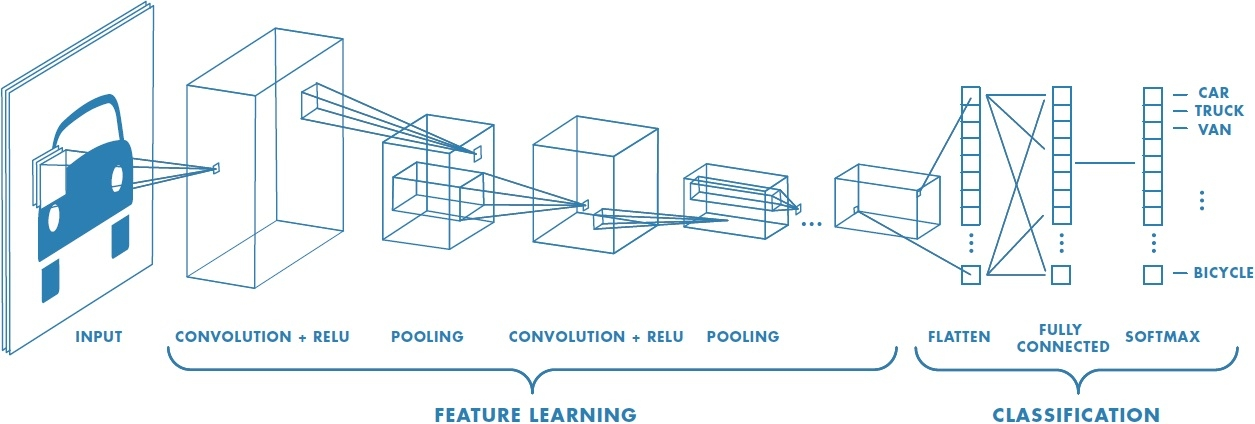
\includegraphics[width=\textwidth]{figures/cnn}
  \caption*{The ``depth'' dimension in the layers shown as cuboids
    corresponds to the number of channels in the output tensor.
    (Figure source: https://www.mathworks.com/solutions/deep-learning/convolutional-neural-network.html)}
\end{figure}

At the end of each filter layer, we typically apply a ReLU activation function. There may be multiple filter plus ReLU layers. Then we have a max pooling layer. Then we have some more filter + ReLU layers. Then we have max pooling again. Once the output is down to
a relatively small size, there is typically a last fully-connected
layer, leading into an activation function such as softmax that
produces the final output. The exact design of these structures is
an art---there is not currently any clear theoretical  (or even
systematic empirical) understanding of how these various design
choices affect overall performance of the network.

The critical point for us is that this is all just a big neural
network, which takes an input and computes an output.  The mapping is
a differentiable function
\note{Well, techinically the derivative does not exist at every point, both because of the ReLU
  and the max pooling operations, but we ignore that fact.}
of the weights, which means we can adjust the weights to decrease the
loss by performing gradient descent, and we can compute the relevant
gradients using back-propagation!

\section{Backpropagation in a simple CNN}

\index{convolutional neural network!backpropagation}
Let's work through a {\em very} simple example of how back-propagation
can work on a convolutional network.   The architecture is shown
below.   Assume we have a one-dimensional single-channel image $X$ of
size $n \times 1 \times 1$, and a single filter $W^1$ of size $k \times 1 \times 1$
(where we omit the filter bias)
for the first convolutional operation denoted ``conv'' in the figure below.
Then we pass the intermediate result $Z^1$
through a ReLU layer to obtain the activation $A^1$,
and finally through a
fully-connected layer with weights $W^2$, denoted ``fc'' below, with no additional
activation function, resulting in the output $A^2$.

\begin{center}
  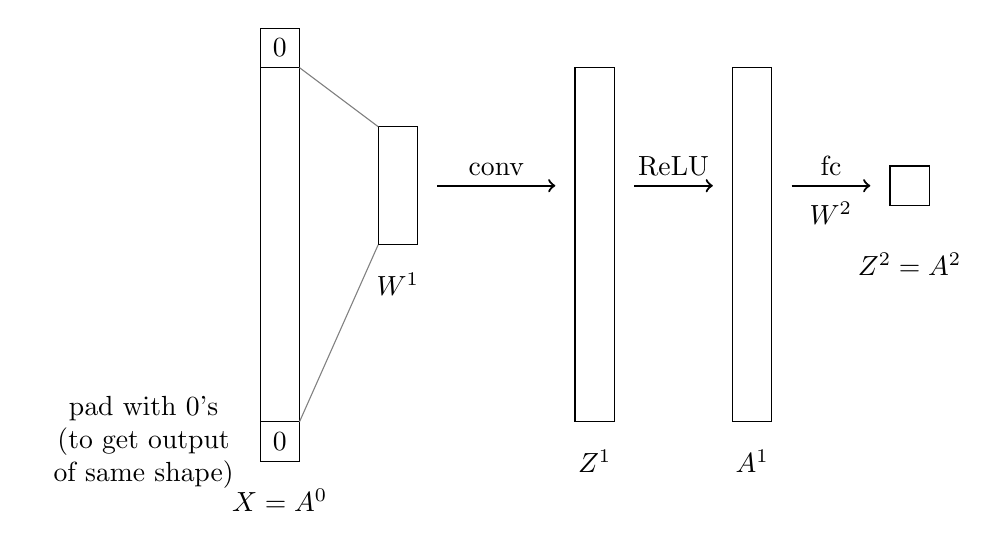
\begin{tikzpicture}[scale=0.5]
    \draw (0,0) rectangle (1,9);
    \node at (.5, -2) {$X = A^0$};
    \draw (0,-1) rectangle (1,0);
    \draw (0,9) rectangle (1,10);
    \node[anchor=center] at (0.5,-.5) {0};
    \node[anchor=center] at (0.5,9.5) {0};
    \node[left] at (0,-0.5) {\begin{tabular}{c}
        pad with 0's \\ (to get output\\ of same shape)\end{tabular}};

    \draw (3,4.5) rectangle (4,7.5);
    \draw[gray] (1,9) -- (3,7.5);
    \draw[gray] (1,0) -- (3,4.5);
    \node at (3.5,3.5) {$W^1$};

    \draw (8,0) rectangle (9,9);
    \node at (8.5,-1) {$Z^1$};

    \draw (12,0) rectangle (13,9);
    \node at (12.5,-1) {$A^1$};

    \draw (16,5.5) rectangle (17,6.5);
    \node at (16.5, 4.0) {$Z^2=A^2$};

    \node at (14.5,5.3) {$W^2$};

    \draw[->,thick] (4.5,6) -- node[above] {conv} (7.5,6);
    \draw[->,thick] (9.5,6) -- node[above] {ReLU} (11.5,6);
    \draw[->,thick] (13.5,6) -- node[above] {fc} (15.5,6);
  \end{tikzpicture}
\end{center}

For simplicity assume $k$ is odd, let the input image $X = A^0$, and
assume we are using squared loss.   Then we can describe the forward
pass as follows:
\begin{align*}
  Z_i^1                        & = {W^1}^TA^0_{[i-\lfloor k/2 \rfloor
  : i + \lfloor k/2 \rfloor]}                                         \\
  A^1                          & = ReLU(Z^1)                          \\
  A^2                          & = Z^2 = {W^2}^T A^1                  \\
  \mathcal{L}_{square}(A^2, y) & = (A^2-y)^2
\end{align*}

\question{Assuming a stride of $1,$ for a filter of size $k$, how much padding do we need to add to the top and bottom of the image? We see one zero at the top and bottom in the figure just above; what filter size is implicitly being shown in the figure? (Recall the padding is for the sake of getting an output the same size as the input.)}

\subsection{Weight update}
How do we update the weights in filter $W^1$?
\[\frac{\partial \text{loss}}{\partial W^1}
  = \frac{\partial Z^1}{\partial W^1}
  \frac{\partial A^1}{\partial Z^1}
  \frac{\partial \text{loss}}{\partial A^1}\]
\begin{itemize}
  \item $\partial Z^1/\partial W^1$ is the $k \times n$
        matrix such that $\partial Z_i^1/\partial W_j^1 =
          X_{i-\lfloor k/2 \rfloor+j-1}$.  So, for example, if $i = 10$,
        which corresponds to column 10 in this matrix, which illustrates
        the dependence of pixel 10 of the output image on the weights, and
        if  $k = 5$, then the
        elements in column 10 will  be $X_8, X_9, X_{10}, X_{11},
          X_{12}$.
  \item $\partial A^1/\partial Z^1$ is the $n \times n$
        diagonal matrix such that
        \begin{eqnarray*}\partial A_i^1/\partial Z_i^1=
          \begin{cases}
            1 & \text{if $Z_i^1 > 0$} \\
            0 & \text{otherwise}
          \end{cases}
        \end{eqnarray*}
  \item $\partial \text{loss}/{\partial A^1}
          = (\partial \text{loss} / {\partial A^2})
          (\partial A^2 / {\partial A^1})
          = 2(A^2 - y)W^2$, an $n \times 1$ vector
\end{itemize}
Multiplying these components yields the desired gradient, of shape
$k \times 1$.

\subsection{Max pooling}
One last point is how to handle back-propagation through a max-pooling
operation.  Let's study this via a simple example.  Imagine
\[y = \max(a_1, a_2)\;\;,\]
where $a_1$ and $a_2$ are each computed by some network.
Consider doing back-propagation through the maximum. First consider the case where $a_1 > a_2$. Then the error %$\delta$ 
value at $y$ is propagated back entirely to the network computing the value  $a_1$. The weights in the network computing  $a_1$ will ultimately be adjusted, and the network computing  $a_2$ will be untouched.
\question{What is $\nabla_{(x, y)} \max(x, y)$ ? }


%%% Local Variables:
%%% mode: latex
%%% TeX-master: "top"
%%% End:
